% Chapter 2

\chapter{Background Theory} % Write in your own chapter title
\label{Chapter2}
\lhead{Chapter 2. \emph{Background Theory}} % Write in your own chapter title to set the page header

\orange
\begin{shaded}
This work takes heavy use of different techniques, theories and tools mostly 
in the context of compiler construction. To simplify the rest of the thesis 
this chapter explains them as far as necessary, thus I may take
them for granted afterwards. As most of the key ideas behind the techniques
will suffice, further details will omitted. 
Interested readers may fall back on the further readings instead. 

\end{shaded}


\yellow
\begin{shaded}
\section{LLVM - The Low Level Virtual Machine}
\label{LLVM}
The Low Level Virtual Machine is a compiler infrastructure designed to optimize
during compiletime, linktime and runtime. Originally designed for C and C++, 
many other frontends for a variety of languages exist by now. The source is 
translated into an intermediate representation (LLVM-IR), which is available 
in three different, but equivalent forms. There is the in-memory compiler IR, 
the on-disk bitcode representation and human readable assembly language.
The LLVM-IR is a type-safe, static single assignment based language,
designed for low-level operations. It is capable of 
representing high-level structures in a flexible way.
Due to the fact that LLVM is built in a modular 
way and can be extended easily, most of the state of the art analysis and
optimization techniques are implemented and shipped with LLVM. Plenty of other
extensions, e.g., Polly, can be added by hand. 

[TODO where to put this ?]
For simplicity most of the examples and argumentation in the thesis will deal 
with C like code instead of LLVM-IR. 

\subsection*{Further Reading}

\begin{itemize}
  \item A Compilation Framework for Lifelong Program Analysis \& Transformation
    \cite{LLVM:CGO04}  
  \item \url{http://www.llvm.org} \nocite{LLVM:Online}
\end{itemize}

\end{shaded}


\orange
\begin{shaded}
\section{The Polyhedral Model}
Polyhedra are mathematical objects living in a vector space of arbitrary 
dimension. They describe a set of points with flat surfaces, thus they can be
seen as solution set of affine inequalities. If they are bounded in all 
dimensions we may speak of polygons instead. 
\lstset{frame=none}
\begin{wrapfigure}[]{r}{0.4\textwidth}
  \centering
  \subfloat[source]{%
    %\begin{minipage}[c][1\width]{%
	   %0.45\textwidth}
	   %\centering%
    \lstinputlisting{Primitives/Code/ExampleLoopNest.c}
    \label{lst:ExampleLoopNest}
    %\end{minipage}
  } 

  \subfloat[polytope model for \ref{lst:ExampleLoopNest}]{%
    %\begin{minipage}[c][1\width]{%
	   %0.45\textwidth}
	   %\centering%
    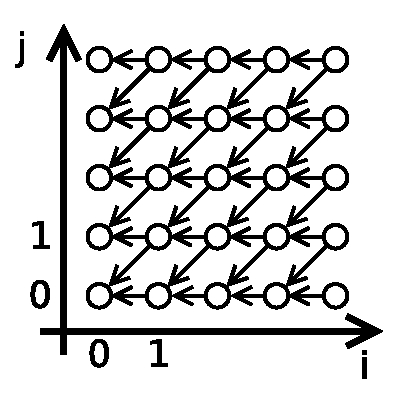
\includegraphics[width=0.3\textwidth]{Figures/ExampleLoopNestPolytope2.eps}
    \label{fig:ExampleLoopNestPolytope}
    %\end{minipage}
  }
  \caption{example loop nest}
  \label{fig:ExampleLoopNest}
\end{wrapfigure}
\resetlst
The polyhedral model is a technique
in compiler construction which relates loop nests with affine bounds and steppings
to polyhedra. The dimension of the surrounding space is determined
by the depth of the loop nests. Each loop corresponds to one dimension but there
might be one more to take the scheduling of the loops into account. Each possible
iteration vectors, a vector containing all induction variables of surrounding 
loops, is represented as a point within the polyhedra. The polyhedral model also contains 
a set of vectors [TODO is it ok to call them vectors ?] to model dependencies
between two iterations, thus between two points. One (composed)
affine transformation within this model may change all dimensions so changes in 
the structure of the loop nest or the scheduling can be described in a
mathematical way. The intention is to analyze and transform the loop nest within
the polyhedral model to find an optimal solution with respect to possible parallelism
or data locality. An example loop nest and the corresponding model
is given by listing \ref{lst:ExampleLoopNest} and 
\ref{fig:ExampleLoopNestPolytope}, respectively. 
Listing \ref{lst:ExampleLoopNestTransformed} shows an equivalent loop nest 
which is now parallelizable in the outermost loop.

\end{shaded}



\lstset{frame=none}
\begin{figure}[htbp]
  \centering
    \lstinputlisting{Primitives/Code/ExampleLoopNestTransformed.c}
  \caption{parallelizable loop nest}
  \label{lst:ExampleLoopNestTransformed} 
\end{figure}
\resetlst

\yellow
\begin{shaded}
\subsection*{Further Reading}
\begin{itemize}
  \item Loop Parallelization in the Polytope Model \cite{Lengauer93loopparallelization}  
  \item PoCC - The Polyhedral Compiler Collection \cite{PoCC:Online}
\end{itemize}

\end{shaded}


\orange
\begin{shaded}
\section{Polly - A Polyhedral Optimizer For LLVM}
\label{Polly}
Exploiting parallelism and data locality to balance the work load and to improve
cache locality are the main goals of the Polly research project. With the 
polytope model, an abstract mathematical representation is used to get optimal
results for a particular objective. It is capable of detection valid loop nests 
which were converted into the polytope model. Employing cloog/isl Polly is able to
perform transformations within the model. The code generation part will create 
LLVM-IR again but if possible with thread level parallelism (via OpenMP) or 
vector instructions (SIMD). Despite the research status, Polly works quite well 
on small examples (listing \ref{lst:ExampleLoopNest} to listing 
\ref{lst:ExampleLoopNestTransformed}) as well as on large benchmarks like the
SPEC 2000 benchmark suite. All parts of Polly this work is directly based on, 
are now explained in more detail as they directly influenced the implementation. 


\subsection{Static Control Parts}
\begin{wrapfigure}[]{r}{0.15\textwidth}
  \centering
  \vspace*{-3mm}
  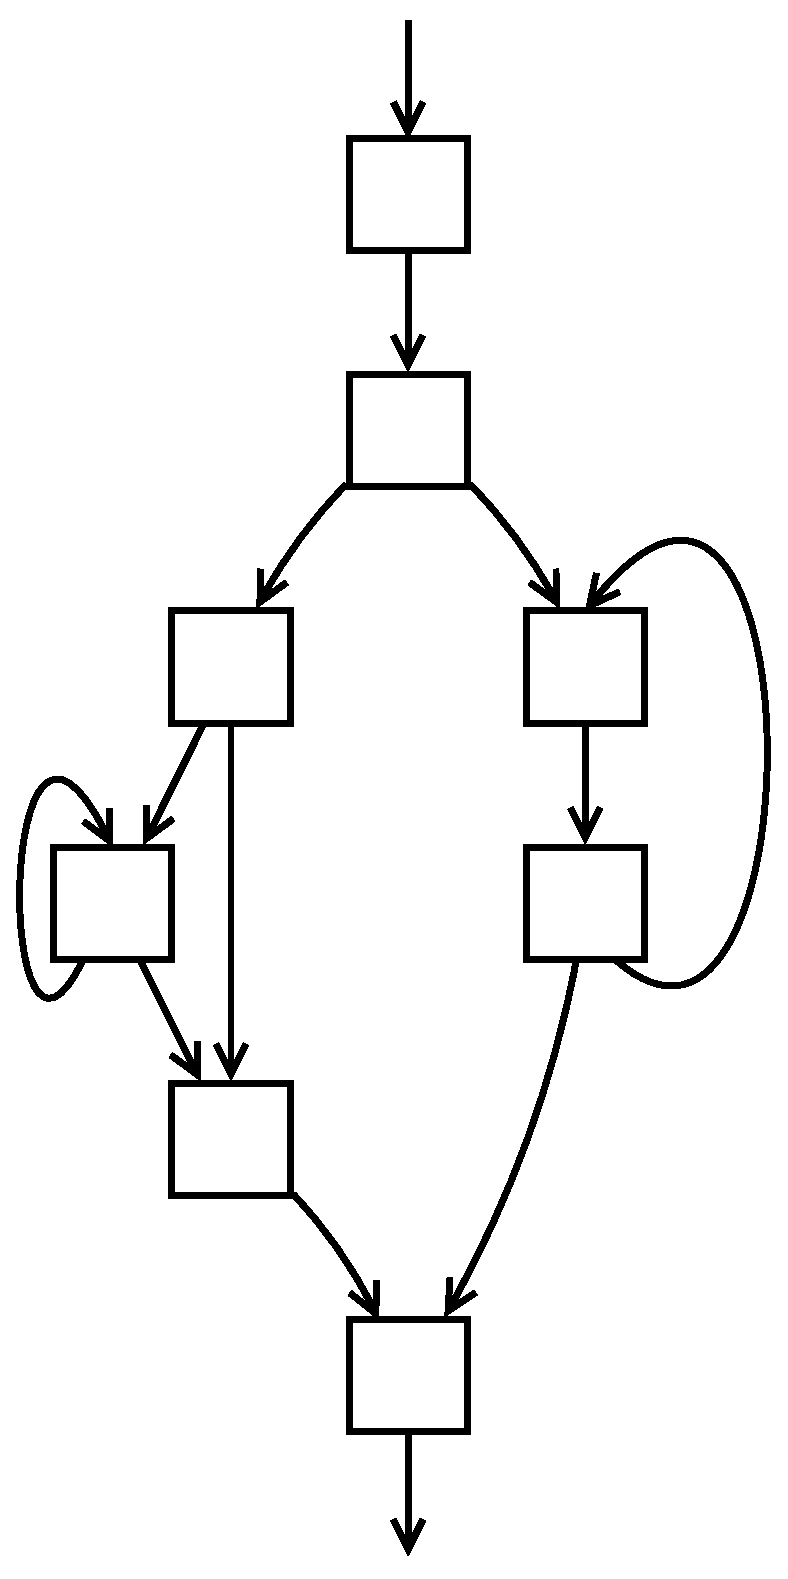
\includegraphics[width=0.15\textwidth]{SimpleRegionCFG.eps}
  \caption{Possible SCoP CFG}
  \label{fig:PossibleSCoPCFG}  
\end{wrapfigure}
Static Control Parts (SCoPs) describe a region which can be safely optimized 
using the polytope model. As this is only possible for SCoPs everything after
the SCoP detection stage may consider the input as such. 
To find the maximal SCoPs within a function, 
all regions are checked for some conditions which need to be fulfilled. 
Starting with the underlying CFG only simple regions with well structured
control flow are considered as SCoPs. This ensures that all loops and branches
are perfectly nested. Other criteria restrict memory accesses or function calls. 
The later one is for example only allowed if the called function does not read
or write any memory location at all, while the former one may not alias with 
other accesses within the SCoP. The trip count of an included loop needs to be
an affine function only depending on loop invariant ``parameters'' and surrounding
induction variables. This restricts the loop bounds to be affine functions too.
As the restriction on a SCoP are quite tight, it is hardly surprising that 
general purpose programs do not contain as many SCoPs as desirable. One goal of
this work was to improve the situation by relaxing some of the restrictions. 
The first part of the evaluation will provide information on the results.

\end{shaded}


\red
\begin{shaded}

\subsubsection{SCoP Detection}



\subsection{Loop Optimizations}

\subsubsection{Parallel Code Generation}

\end{shaded}



\begin{figure}[htbp]
  \centering
  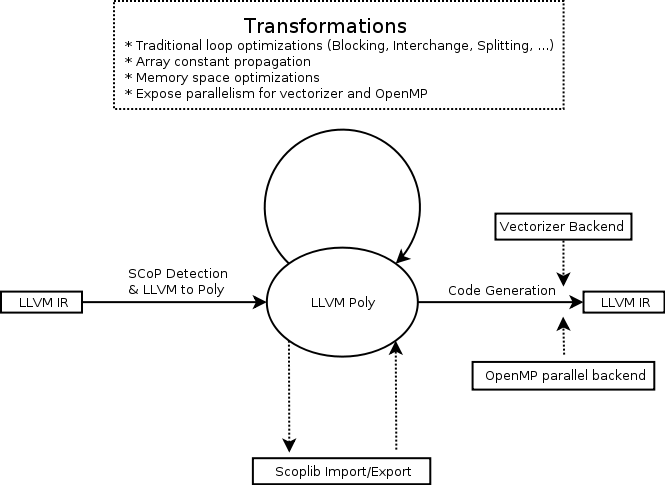
\includegraphics[width=0.9\textwidth]{architecture.png}
  \caption{Pollys architecture \cite{Polly:Online}}
  \label{fig:PollyArchitecture}  
\end{figure}


\yellow
\begin{shaded}
\subsection*{Further Reading}

\yellow
\begin{itemize}
  \item Polly - Polyhedral optimization in LLVM \cite{grosser.11.impact}  
  \item Enabling Polyhedral Optimizations in LLVM \cite{grosser:thesis}
  \item A Framework for Automatic OpenMP Code Generation \cite{raghesh2011framework}
  \item \url{http://polly.llvm.org} \nocite{Polly:Online}
\end{itemize}

\end{shaded}


\red
\begin{shaded}
\section{Sambamba - A Framework For Adaptive Program Optimization}
As an extension for LLVM the \textit{Sambamba} compiler framework is designed to
allow runtime analyses and (speculative) optimization.
Furthermore these optimization can create and refine runtime profiles which
are used to recalibrate and specialize the (speculative) execution. Method 
versioning allows conservative and speculative 
versions of a method to be stored and switched during runtime. 
%But both can profit from specialization at runtime. 
%especially after conflicting speculation.
%Based on the LLVM suite, Sambamba uses the shipped JIT compiler 
%and a software transactional memory system to secure
%speculative execution. 
Written in a completely modular way, Sambamba extensions consist 
of a static part (compiletime) and a dynamic one (runtime). 
Both extension parts can use Sambamba to store information,
collected at the corresponding time, accessible for the dynamic part at 
runtime.
%In the context of speculation and profiling, Sambamba can be used to store
%several version of a method which can be generated by one of the two parts.
Profiling combined with the method versioning system allows runtime interactions
to explore more parallelism or minimize the overhead in case of misspeculation. 

\subsection{ParCFGs}

\subsection{Parallelizer}

\subsection*{Further Reading}
\begin{itemize}
  \item Sambamba: A Runtime System for Online Adaptive Parallelization \cite{DBLP:conf/cc/StreitHZH12}  
  \item \url{http://www.sambamba.org} \nocite{StreitHZH12:Online}
\end{itemize}

\end{shaded}


